\section{Redis}

In this chapter, we will explore Redis performance. Initially, we will focus on performance under the default configuration. Subsequently, we will explore the scalability of Redis. We will focus on the impact of multiple instances running simultaneously under various load configurations. Unless otherwise stated, all benchmarks will be performed such that they meet the desired Quality of Service (QoS) defined as having 99th percentile latency under 1 millisecond.

\subsection{Out of the Box Performance}
Firstly, let us focus on the performance characteristics Redis achieves without any special configuration enabled. Once deployed to a server, a Redis server can be started with the following:
\begin{lstlisting}
redis redis.conf --port 11120
\end{lstlisting}

The \texttt{redis.conf} refers to a configuration file which is part of the official distribution \cite{RedisConfiguration}. Any arguments prefixed with \texttt{--} will overwrite the settings inside \texttt{redis.conf}. In our case, we are setting the port to listen on 11120. Otherwise, all configuration remains unmodified.

The clients are setup in order to produce an increasing load on Redis. In order to do this, we increase the number of connections each client will utilize to send requests to the Redis server. The number of connections is increased at a constant rate of 1. Note that we utilize the \texttt{-P} argument to specify we are interested in benchmarking Redis.

\begin{lstlisting}
memtier -s nsl200 -p 11120 -c <connection_count> -t 2 -P redis
--random-data
--key-minimum=100
--key-maximum=10000
\end{lstlisting}

/subsubsection{Latency vs Throughput}

Firstly, let us consider the relationship between latency and throughput.

\begin{figure}[h]
    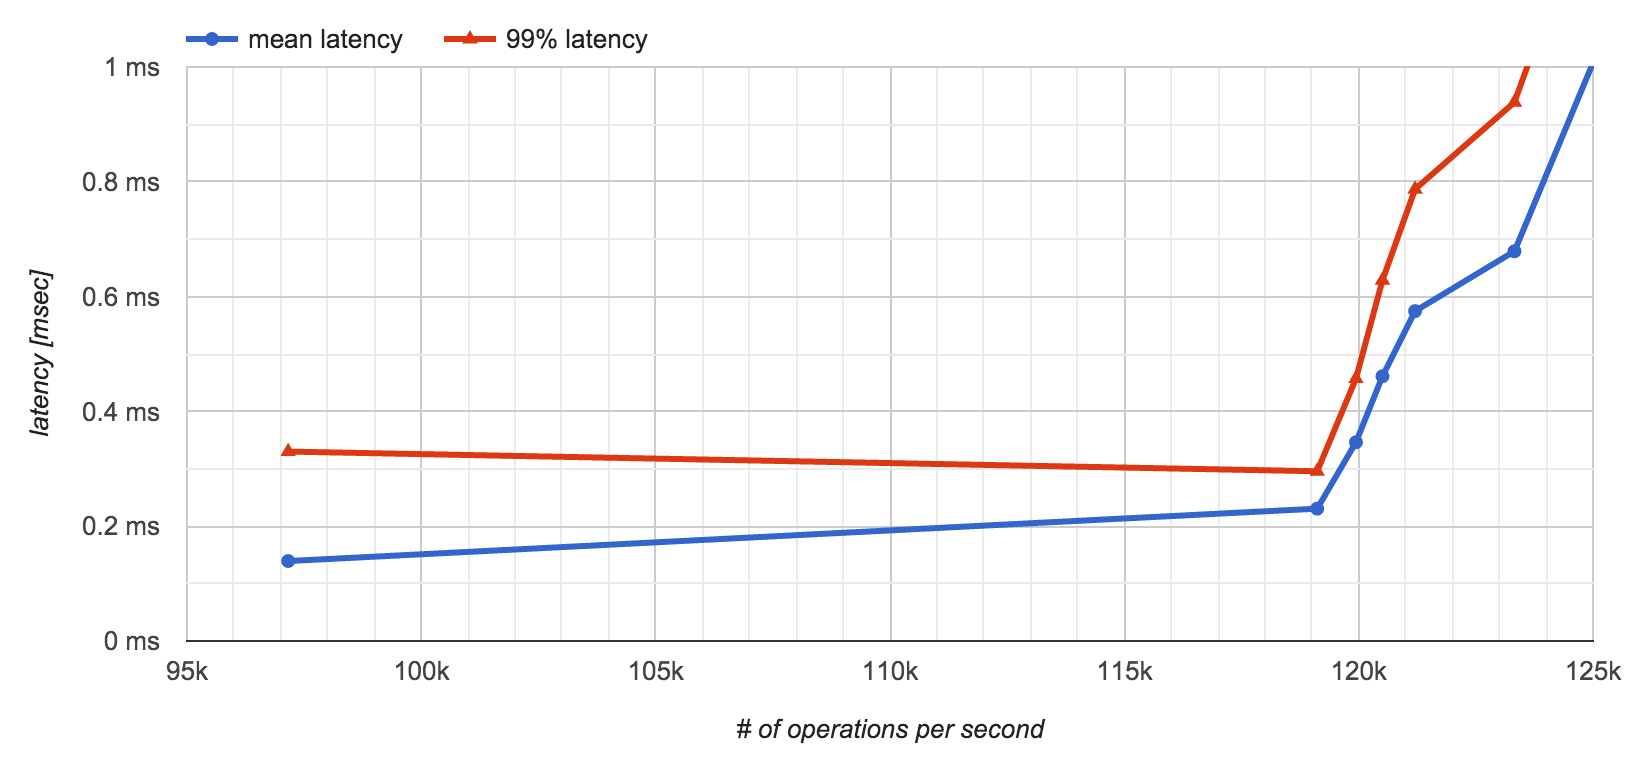
\includegraphics[width=\textwidth]{./res/6_default_latency_ops.png}
    \caption{Redis: Throughput vs Mean and 99th percentile latency}
    \label{fig:redis-default-latency-ops}
\end{figure}

Figure \ref{fig:redis-default-latency-ops} shows the relationship between mean and 99th percentile latency on the vertical axis and the number of operations per second on the horizontal axis. The graph has been trimmed to show only data which satisfies the QoS requirements. We can observe that the number of operations Redis processes increases steadily until it reaches 119k requests per second at which point a further increase in throughput comes at a disproportionately grater cost in latency. The peak throughput observed under the QoS requirements is 125,000 requests per second.

/subsubsection{CPU Utilization}

Secondly, analyzing CPU utilization of Redis provides insights into the relative requirements of the system in relation to the underlying operating system.

\begin{figure}[h]
    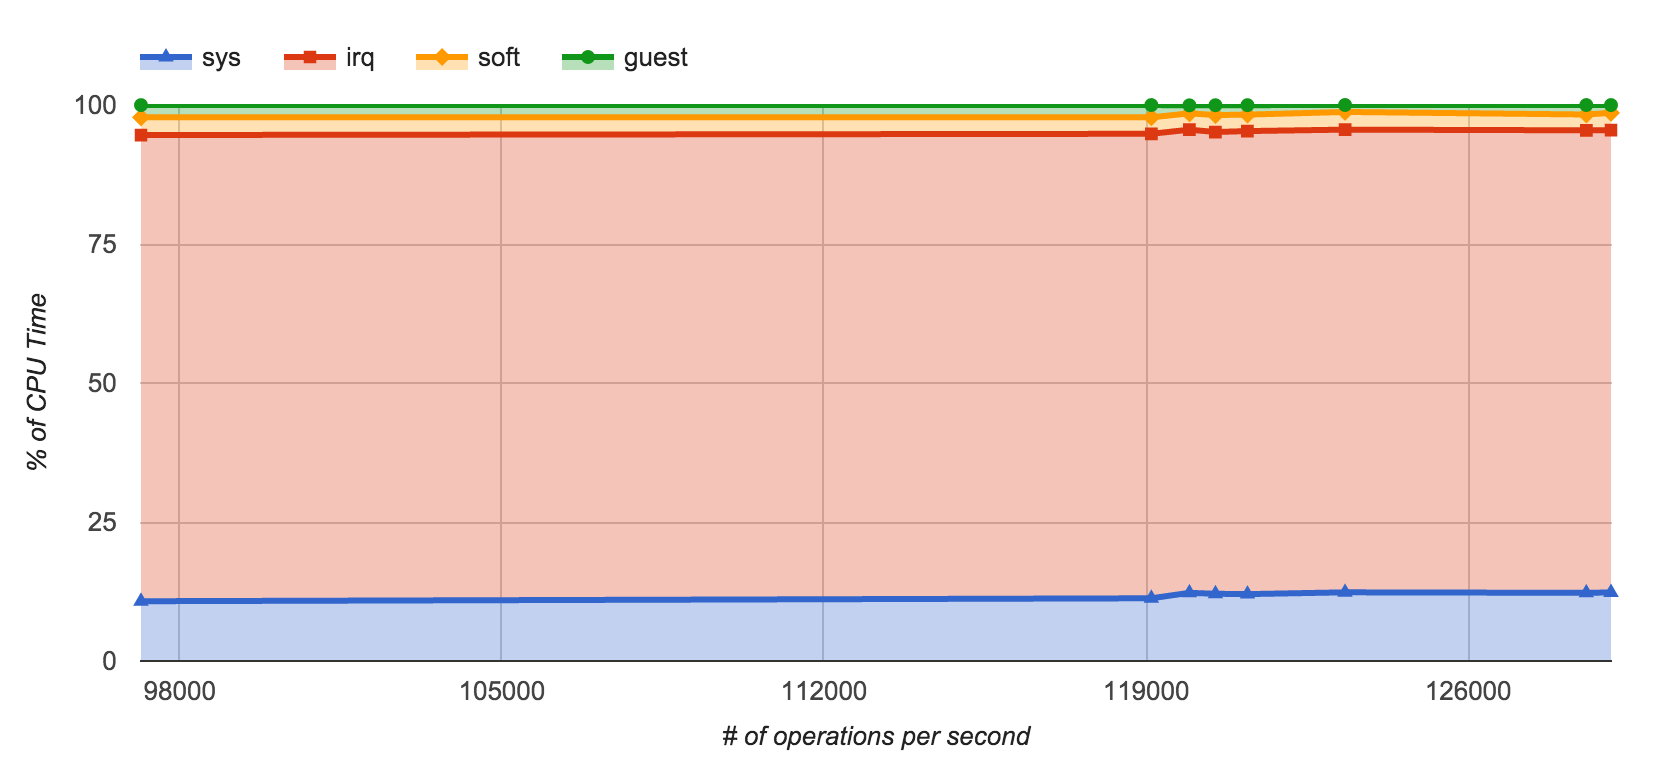
\includegraphics[width=\textwidth]{./res/6_default_cpu.png}
    \caption{Redis: CPU Utilization}
    \label{fig:redis-default-cpu}
\end{figure}

Figure \ref{fig:redis-default-cpu} outlines CPU utilization in terms of time spent in various regions. We can observe that servicing hardware interrupts (irq) takes up majority - 83 percent - of the total time. This is due to processing interrupts from the network card. The system requires around 10 percent of time while Redis itself only requires around 2 percent. Remaining time is spent handling software interrupts - about 3 percent. From the data above, Redis is not CPU intensive on its own, rather it is network intensive and spends most time receiving and dispatching network requests.


Redis, with default configuration, is capable of delivering around 125k requests per second and operates under heavy usage of the underlying network protocol.


\subsection{Multiple Redis Instances}
\label{sec:multiple-redis-instances}
Redis is a single threaded application, in order to increase performance, we can run multiple Redis instances simultaneously to increase the number of CPU cores utilized.

The benchmark configuration for this section considers a scenario where a fixed load generated by clients is partitioned across an increasing number of Redis instances. In particular, the load exerted in the case of a single instance may not meet required QoS, however, it is required to be able to show the trend.

In order to perform the benchmark, we can setup the \texttt{i} instances of Redis, each accepting connections on a distinct port. These instances are separate applications and do not operate under shared memory model. We can start the Redis servers with the following script to launch \texttt{i} instances of Redis on ports starting at 11120.

\begin{lstlisting}
for j in [1..i]
    redis-server redis.conf --port (11120 + j)
\end{lstlisting}

When launching the benchmark clients, we need to take care maintain the level of load the same while spreading the load onto more instances. Let us assume that we can exert load \texttt{l} then if there \texttt{i} instances of Redis then for each benchmarking server (host), we need to exert \texttt{l / i} proportionate load per each Redis instance. Additionally, the key range should be reduced proportionately to the number of instances as in a real scenario running multiple instances would lead to a partitioned key space. Subsequently, as the load is partitioned, we spawn \texttt{i} instances of the Memtier benchmark on each benchmarking host. This results in maintaining a stable load while partitioning the server into multiple instances.

Therefore, each Memtier client can be launched with the following script where \texttt{round()} is a rounding function. Whenever we cannot partition the load precisely, we generate two test scenarios and apply a \texttt{ceiling} and \texttt{floor} function, averaging the results.

\begin{lstlisting}
for j in [1..i]
    memtier -s nsl200 -p 11120 -c round(16 / j) -t 1 -P redis
        --random-data
        --key-minimum=100
        --key-maximum=round(10000 / j)
\end{lstlisting}

\subsubsection{Latency and Throughput vs Instance Count}

Firstly, in this section we consider the impact of increasing the number of Redis instances on a single machine. Note that the host used as a server has 6 CPUs.

\begin{figure}[h]
    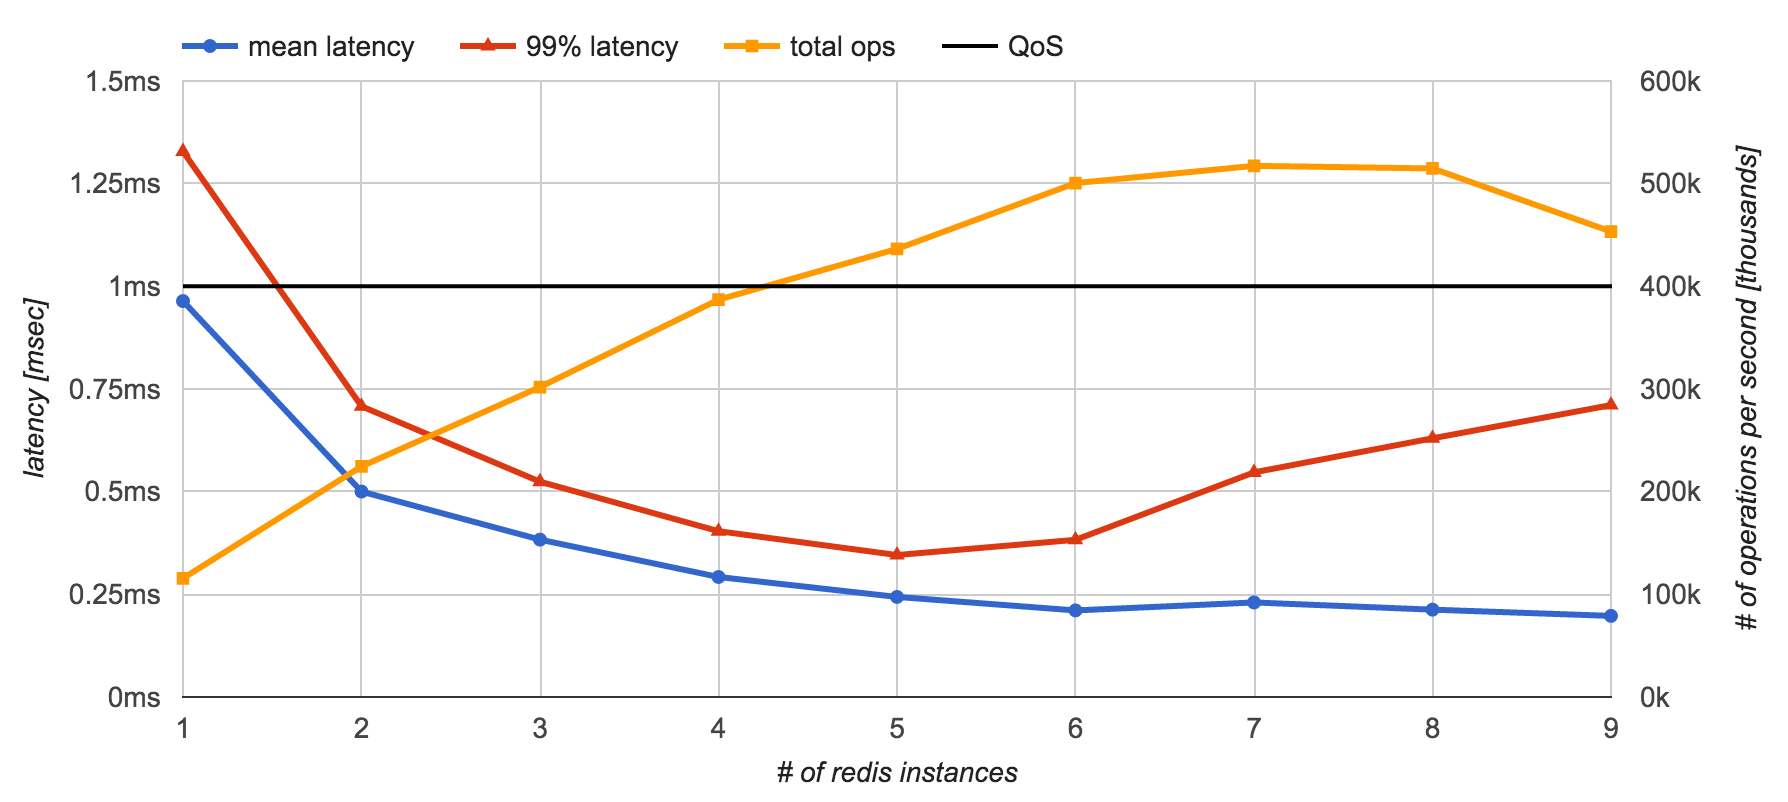
\includegraphics[width=\textwidth]{./res/6_instances_latency_ops.png}
    \caption{Redis Instances: Latency, Throughput vs Number of instances}
    \label{fig:redis-instances-latency-ops}
\end{figure}

Figure \ref{fig:redis-instances-latency-ops} displays latency and 99th percentile latency on the left vertical axis, the throughput on the right vertical axis against the number of instances on the horizontal axis.

As the number of processes increases, both mean and 99th percentile latency decrease steadily. The 99th percentile latency reaches a minimum at 5 processes and rises as number of processes is increased further. The minimum 99th percentile latency achieved is around 0.345ms. The mean continues to decrease at a much slower pace beyond it's minimum at 6 processes.

Additionally, as the number of instances increases, throughput increases. Throughput increases linearly until 6 instances are reached at which point the rate of increase decreases. Beyond 8 instances, the throughput begins to decrease. Between 6 and 8 instances, we are able to achieve close to 500k requests per second.

The QoS target is achieved in all but the 1 instance scenario. Furthermore, we can observe that Redis manages to scale quite well by increasing the number of instances until we reach 6 instances. Beyond 6 instances, the throughput degrades and the 99th percentile begins to climb again. The best balance of throughput and minimal 99th percentile latency is when running 6 instances, the same as the number of CPU cores available.

\subsubsection{CPU Utilization vs Instance Count}
Let us now explore the impact of running multiple Redis instances simultaneously on the CPU utilization.

\begin{figure}[h]
    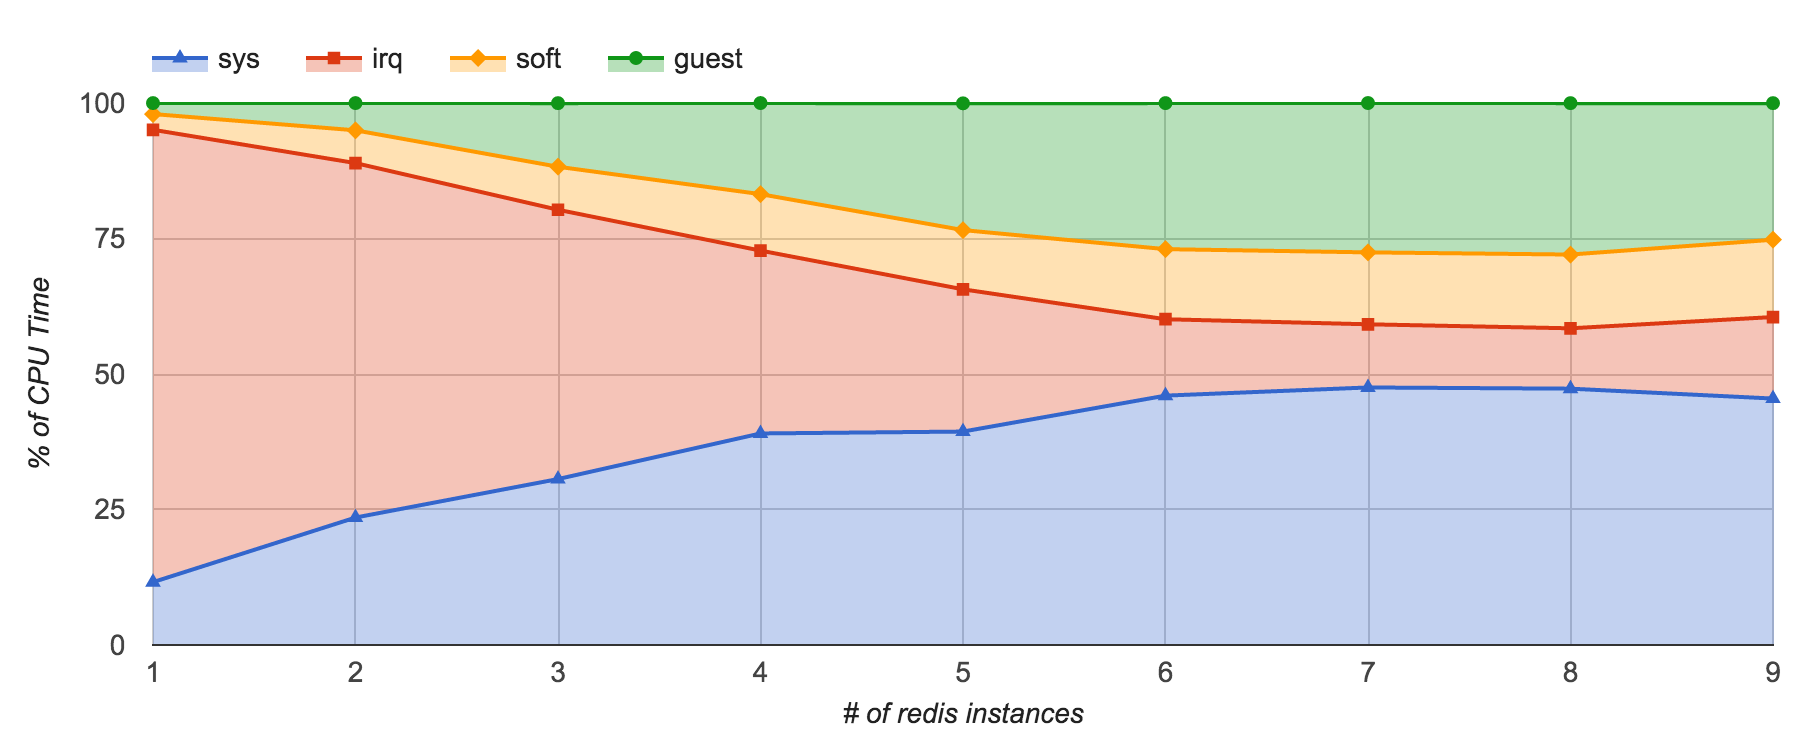
\includegraphics[width=\textwidth]{./res/6_instances_cpu.png}
    \caption{Redis Instances: CPU Utilization vs Number of Instances}
    \label{fig:6_instances_cpu.png}
\end{figure}

From \ref{fig:6_instances_cpu.png} we can see that as we increase the number of instances, the CPU usage of Redis (\textit{guest}) increases until we reach 6 instances at which point it flattens out. Similarly, the resources required by OS (\textit{sys}) to support the increasing number of instances grows until 6 processes, further increase in the number of instances does not result in increased resource usage. The amount of context switching (soft) required increases as the number of instances increases and remains constant beyond 6 instances. Conversely, the time spent processing hardware interrupts from the network decrease, this is due to batching at the network layer as the number of instances increases.

Despite the increased resource requirements by Redis, it still only accounts for about 27 percent CPU usage at 6 processes with majority of the CPU time spent in the operating system and or networking.


By spawning multiple instances of Redis, we have been able to dramatically increase the overall performance of the server. The peak throughput observed is at 500k requests per second while the mean and 99th percentile latency remains within the QoS restrictions.


\subsection{Pinned Redis Instances}

In the previous section we have observed that the performance of a Redis server can be greatly increased by spawning multiple Redis instances simultaneously. Pinning processes to distinct cores is suggested to improve tail latency \cite{leverich2014reconciling}. In this section, we examine the effect process pinning has on the performance of Redis. A Redis thread can be pinned to a unique core through the use of \texttt{taskset} utility as follows:

\begin{lstlisting}
taskset -pc <redis_pid> <core_id>
\end{lstlisting}

The Redis and benchmark configuration used is the same in section \ref{sec:multiple-redis-instances}, that is, the number of Redis processes is linearly increased while maintaining the same level load.

\begin{figure}[h]
    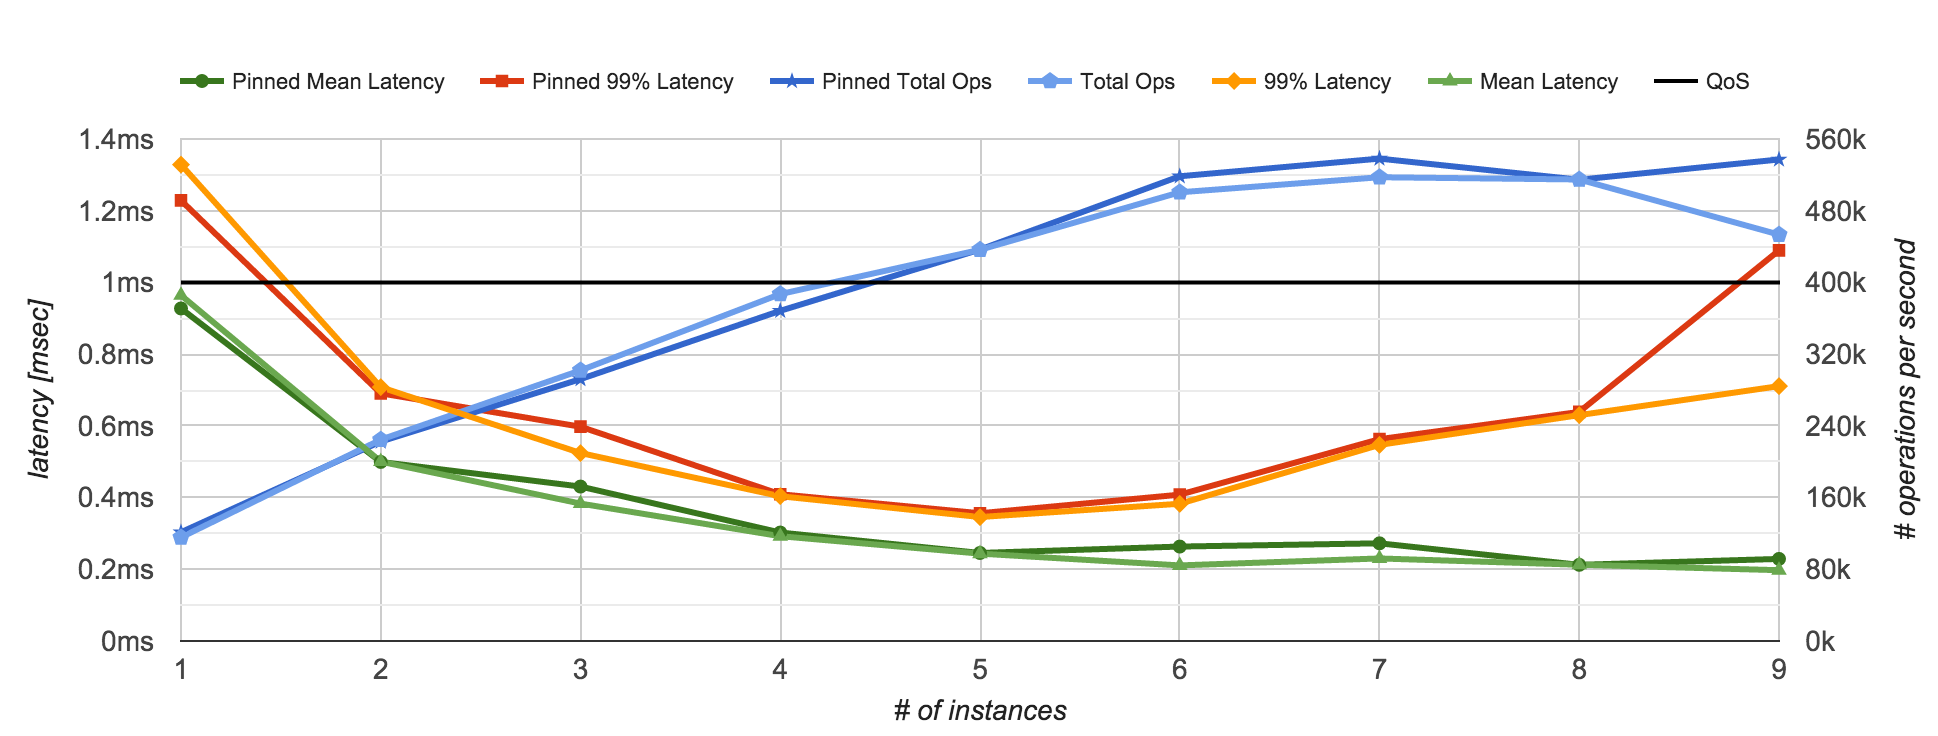
\includegraphics[width=\textwidth]{./res/6_pinned.png}
    \caption{Redis Instance Pinning: Instances vs Latency and Throughput}
    \label{fig:6_pinned.png}
\end{figure}